\documentclass[preview]{standalone}

\usepackage{amsmath}
\usepackage{amssymb}
\usepackage{bettelini}
\usepackage{stellar}
\usepackage{definitions}
\usepackage{makecell}
\usepackage{tikz}
\usetikzlibrary{arrows,matrix}

\begin{document}

\id{cyclid-groups}
\genpage

\section{Cyclid groups}

\begin{snippetdefinition}{cyclic-group-definition}{Cyclic Group}
    Let \(G\) be a \group. For any element \(g\) in \(G\),
    the \textit{cyclic group} is the \group generated by \(g\).
\end{snippetdefinition}

\begin{snippetcorollary}{cyclic-is-abelian}{Cyclic groups are abelian}
    Let \(G\) be a \group. If \(G\) is \cyclicgroup[cyclic], then it is \abeliangroup[abelian].
\end{snippetcorollary}

\begin{snippetproof}{cyclic-is-abelian-proof}{cyclic-is-abelian}{Cyclic groups are abelian}
    A generated \subgroup is \abeliangroup[abelian] \ifandonlyif
    the elements of its generator commute. Since the \cyclicgroup
    has only one element, it commutes with itself.
\end{snippetproof}

\begin{snippettheorem}{subgroups-of-cyclic-are-cyclic}{Subgroups of cyclic groups}
    Any \subgroup of a \cyclicgroup is \cyclicgroup[cyclic].
\end{snippettheorem}

\begin{snippetproof}{subgroups-of-cyclic-are-cyclic-proof}{subgroups-of-cyclic-are-cyclic}{Subgroups of cyclic groups}
    Let \((H, \circ) \subgroupleq (G, \circ) = \gengrp{g}\).
    The \subgroup \(H\) is formed by (some) power of \(g\). We consider the following subset:
    \[
        S = \{ n \in \integers \suchthat g^n \in H \}
    \]
    We have that \(0 \in S\) as \(g^0 = 1 \in H\).
    If \(S = \{0\}\), \(H=\{1\}\) and we are done (it is generated by \(1\)).
    If \(S \neq \{0\}\), there are \(n\neq 0 \in S\).
    This means that \(g^n \in H\).
    Since \(g^n \in H\), we also have \(g^{-n} \in H\), meaning \(-n\in S\).
    Since \(n \neq 0\), either \(n\) or \(-n\) is positive.
    This implies that \(S\) contains some positive integers.
    Let \(d\) be the smallest positive integer in \(S\).
    This means that \(g^d \in H\) and if \(0<k<d\), then \(g^k \notin H\).
    We now show that \(g^d\) generates \(H\), meaning that every element of \(H\)
    is a power of \(g^d\). The powers of \(g^d\)
    are of the form \(g^{dn}\) with \(n \in \integers\).
    Let \(g^m \in H\). We want to show that \(m=dn\) for some \(n\).
    We thus divide \(m\) by \(d\). We get
    \begin{align*}
        m &= dq + r \qquad 0\leq r < d \\
        g^m &= g^{dq+r} = {(g^d)}^r \circ g^r
    \end{align*}
    We want to show that \(g^r = 1\). Now, \(g^r = {(g^d)}^{-q} \circ g^m\).
    Both terms are in \(H\), so \(g^r \in H\). By definition of \(d\), \(r=0\)
    since we cannot have \(0 < r < d\) such that \(r\in S\).
    Finally \(g^m = g^{dq}\).
\end{snippetproof}

\begin{snippetproposition}{cyclic-group-powers}{Cyclic groups powers}
    Let \(G\) be a \group. For any element \(g\) in \(G\),
    the \cyclicgroup
    \[
        \gengrp{g} = \{ g^k \suchthat k \in \naturalnumbers \}
    \]
\end{snippetproposition}

\subsection{Period of a cyclic group}

\begin{snippetdefinition}{cyclic-group-period-definition}{Cyclic group period}
    Let \((G, \circ) = \gengrp{g}\) be a \cyclicgroup.
    The \emph{period} of \(g\)
    is the smallest positive integer \(d\) such that \(g^d = 1\)
    and is denoted as \(|g|\).
    We define \(|g| = \infty\) if all the powers of \(g\) are distinct.
\end{snippetdefinition}

\begin{snippettheorem}{cyclic-group-periodic-finite}{Finite cyclic group}
    A \cyclicgroup is \cyclicperiod[periodic] \ifandonlyif it is finite.
    % TODOURGENT or has finite period
    The \cyclicperiod is the order of the \group.
\end{snippettheorem}

\begin{snippetproof}{cyclic-group-periodic-finite-proof}{cyclic-group-periodic-finite}{Finite cyclic group}
    Let \((G, \circ)\) be a \cyclicgroup. We know that
    \[
        (G, \circ) = \{ g^n \suchthat n \in \integers \}
    \]
    Let \(m,n \in\integers\) such that \(m\neq n\).
    In the case where \(g^m \neq g^n\), the \group is infinite.
    If this does not happen, there exist \(m\) and \(n\) such that \(g^m = g^n\).
    Without loss of generality, assume \(n>m\).
    We thus have \(g^{n-m} = g^n \circ g^{-m} = g^m \circ g^{-m} = 1\).
    Thus, there exist \(n-m>0\) such that \(g^{n-m} = 1\). This always happens
    when two different powers give the same element.
    Let \(d\) be the smallest positive integer such that
    \(g^d = 1\).
    We now show that \(g^n = g^k\) \ifandonlyif \(h \equiv k \pmod{d}\).
    We divide \(h-k\) by \(d\), and we get
    \begin{align*}
        h-k = qd + r \qquad 0 \leq r < d
    \end{align*}
    We thus have \(g^h = g^k \circ g^{qd} \circ g^r\).
    Since \(g^qd = 1^q = 1\), \(g^h = g^k \circ g^r\).
    Thus, \(g^h = g^k\) \ifandonlyif \(g^r = 1\),
    which only happens when \(r=0\) by the definition of \(d\),
    meaning \(h\equiv k \pmod{d}\).
    It follows that \(\gengrp{g}\) is finite and it contains
    exactly \(d\) elements.
    We may also note that \(|g| = 1 \iff g=1\).
\end{snippetproof}

\begin{snippettheorem}{order-of-power-of-group-element-theorem}{Order of Power of Group Element}
    Let \((G, \circ)\) be a \group and let \(|g| = d\). Then,
    \[ |g^n| = \frac{d}{\gcd(d,n)} \]
\end{snippettheorem}

\begin{snippetproof}{order-of-power-of-group-element-proof}{order-of-power-of-group-element-theorem}{Order of Power of Group Element}
    Let \(d=d'\gcd(d,n)\) and \(n=n'(d,n)\).
    The values \(n'\) and \(d'\) are \coprime. We need to show that \(|g^n| = d'\).
    We have
    \[
        {(g^n)}^{d'} = g^{nd'} = g^{n'\gcd(d,n)d'} = g^{dn'}
        = {(g^d)}^{n'} = 1^{n'} = 1
    \]
    We thus showd that \(|g^n|\) divides \(d'\).
    Let \(k \in\integers\) such that \({(g^n)}^k = 1\), meaning \(g^{nk} = 1\).
    This happens \ifandonlyif \(d \divides nk\), meaning \ifandonlyif there exist \(h\in\integers\)
    such that \(dh = nk\). However, \(hd'\gcd(d,n) = \gcd(d,n)n'k\) and thus \(d'h = n^k\).
    Since \(d'\) and \(n'\) are \coprime, this happens \ifandonlyif \(d' \divides k\) and thus
    \({(g^n)}^k = 1\) \ifandonlyif \(k\) is a multiple of \(d\), which is the \cyclicperiod.
\end{snippetproof}

\begin{snippet}{order-of-power-of-group-element-note}
    Note that \(|g^n| = d \iff \gcd(n,d)=1\). This means that \(g^n\) generates a \subgroup[subgroups]
    of \(\gengrp{g}\) of order \(d\), that is \(\gengrp{g}\) itself.
    This means that the elements of the form \(g^n\) with \(\gcd(n,d) = 1\)
    are alternative generators of \(\gengrp{g}\).
    The amount of these elements is \(\eulertotient(d)\).
\end{snippet}

\begin{snippettheorem}{unique-subgroups-for-every-divisor-of-cyclic-order-theorem}{}
    Let \((G, \circ) = \gengrp{g}\) be a finite \cyclicgroup
    of order \(d\). For every divisor \(n\) of \(d\), there exist a unique
    \subgroup of \((G, \circ)\) of order \(n\). If \(H\) and \(K\)
    are \subgroup[subgroups] of \((G, \circ)\)
    with order \(m\) and \(n\) respectively, then \(H \subgroupleq K \iff m \divides n\).
\end{snippettheorem}

\begin{snippetproof}{unique-subgroups-for-every-divisor-of-cyclic-order-proof}{unique-subgroups-for-every-divisor-of-cyclic-order}{}
    Let \(n\) be a divisor of \(d\).
    We want to show that there exist at least a \subgroup of \((G, \circ)\)
    of order \(n\). We know that 
    \[
        |g^k| = \frac{d}{\gcd(d,k)}
    \]
    so we choose, for instance, \(k=\frac{d}{n}\), we thus get
    \[
        |g^k| = \frac{d}{\gcd(d, d/n)} = \frac{d}{d/n} = n
    \]
    We now show that if \(|g^h| = n\), then \(\gengrp{g^h} = \gengrp{g^{k}}\),
    which means that the \subgroup of order \(n\) is unique.
    We have \[ \frac{d}{\gcd(d,n)} = n \]
    meaning \(\gcd(d,h) = \gcd(d, k) = k\).
    In particular, \(k \divides h\). Thus,
    \(g^h\) is a power of \(g^k\), meaning that \(g^h \in \gengrp{g^k}\),
    from which it follows that \(\gengrp{g^h} \subgroupleq \gengrp{g^k}\).
    However, \(|\gengrp{g^h}| = |\gengrp{g^k}|\), meaning \(\gengrp{g^h} = \gengrp{g^k}\).
    We now show that if \(H\) and \(K\) are \subgroup[subgroups] of \((G, \circ)\), 
    we have \(H \subgroupleq K \iff |H| \divides |K|\).
    We just proved that if \(H \subgroupleq K\), then \(|H| \divides |K|\).
    Viceversa, if \(|H| \divides |K|\), we know that there exist a \(H' \subgroupleq K\)
    of order \(|H|\). However, \(H\) and \(H'\) are \subgroup[subgroups] of \((G, \circ)\)
    of the same order, so they are the same \(H=H'\subgroupleq K\).
\end{snippetproof}

\plain{In an arbitrary finite group, there do not necessarily exist subgroups of orders of every divisor
of the order of the group. There could exist different subgroups of the same order.
For example, the Klein groups (which is not cyclic) has precisely three distinct subgroups of order 2.}

\begin{snippet}{finite-cyclic-subgroups-orders}
    Let \((G, \circ)\) be a finite \cyclicgroup of order \(d\)
    and let \(n\) a divisor of \(d\). There are exactly \(\eulertotient(n)\)
    elements of order \(n\).
    All these elements are in a unique \subgroup of \((G, \circ)\)
    of order \(n\), which contains exactly \(\eulertotient(n)\) elements of period \(n\)
    for every \(n \divides d\). Furthermore, \((G, \circ)\) contains exactly \(n\) elements
    of period \(k\) where \(k \divides n\) (they are all the elements of the only \subgroup or order \(n\)).
\end{snippet}

\begin{snippetcorollary}{integer-sum-of-eulertotient}{}
    Let \(d\) be a positive integer.
    \[
        \sum_{n \divides d} \eulertotient(n)
    \]
\end{snippetcorollary}

\begin{snippetproof}{integer-sum-of-eulertotient-proof}{integer-sum-of-eulertotient}{}
    Consider a \cyclicgroup of order \(d\).
    For every divisor \(n\) of \(d\), it contains exactly \(\eulertotient(n)\)
    elements of \cyclicperiod \(n\). Since the \group contains
    \(d\) elements, the thesis directly follows by summing the amount of its elements.
\end{snippetproof}

\subsection{Subgroups of infinite cyclic groups}

\begin{snippetproposition}{subgroups-of-infinite-cyclic-groups}{Subgroups of infinite cyclic groups}
    The \cyclicgroup[cyclic] \subgroup[subgroups]
    of an infinite \cyclicgroup are infinite, except
    for the trivial case.
\end{snippetproposition}

\begin{snippetproof}{subgroups-of-infinite-cyclic-groups-proof}{subgroups-of-infinite-cyclic-groups}{Subgroups of infinite cyclic groups}
    Let \((G, \circ) = \gengrp{g}\)
    where \(|g| = \infty\).
    We know that the \subgroup[subgroups] are of the form
    \(\gengrp{g^n}\) for \(n\in\integers\).
    We want to study \(|g^n|\).
    We have that \({(g^n)}^k = 1\) \ifandonlyif \(g^nk = 1\),
    which happens \ifandonlyif \(nk=0\).
    if \(n=0\), this happens for every \(k\) (\(\gengrp{g^n}\) is the trivial case).
    If \(n\neq 0\), this happens \ifandonlyif \(k=0\), meaning \(|g^n| = \infty\).
\end{snippetproof}

\begin{snippetproposition}{infinite-cyclic-groups-comparison}{}
    Let \(\gengrp{g} = (G, \circ)\) be a \cyclicgroup where \(|g|=\infty\).
    We have that
    \[\gengrp{g^n} \subgroupleq \gengrp{g^m} \iff m \divides n\]
    and
    \[
        \gengrp{g^n} = \gengrp{g^m} \iff m=n \lor m=-n
    \]
    In particular, \((G, \circ) = \gengrp{g} = \gengrp{g^{-1}}\).
\end{snippetproposition}

\begin{snippetproof}{infinite-cyclic-groups-comparison-proof}{infinite-cyclic-groups-comparison}{}
    We now want to compare \(\gengrp{g^n}\)
    and \(\gengrp{g^m}\). The two are the same if
    if the generator is in both \subgroup[subgroups].
    We have that \(\gengrp{g^n} \subgroupleq \gengrp{g^m}\)
    \ifandonlyif there exist \(h\in\integers\) such that \(g^n = {(g^m)}^h = g^{mh}\).
    Since \(|g| = \infty\), this happens \ifandonlyif \(n=mh\), that is \ifandonlyif
    \(m\divides n\).
\end{snippetproof}

\begin{snippet}{cyclic-subgroups-illustration}
    \begin{center}
        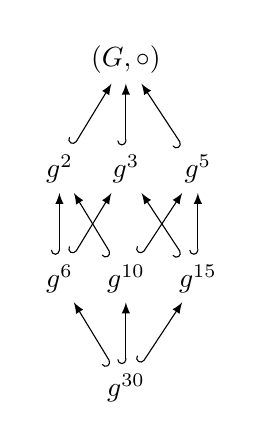
\begin{tikzpicture}[scale=2]
            \matrix [matrix of math nodes, row sep = 0.8cm]
                {
                                      & |(1)| {(G, \circ)}               &  \\
                |(2)| {\gengrp{g^{2}}} & |(3)| {\gengrp{g^{3}}}   & |(5)|  {\gengrp{g^{5}}} \\
                |(6)| {\gengrp{g^{6}}} & |(10)| {\gengrp{g^{10}}} & |(15)| {\gengrp{g^{15}}} \\
                                      & |(30)| {\gengrp{g^{30}}} &  \\
                };
            \draw[right hook-latex] (2)--(1);
            \draw[right hook-latex] (3)--(1);
            \draw[right hook-latex] (5)--(1);

            \draw[right hook-latex] (6)--(2);
            \draw[right hook-latex] (10)--(2);

            \draw[right hook-latex] (6)--(3);
            \draw[right hook-latex] (15)--(3);

            \draw[right hook-latex] (10)--(5);
            \draw[right hook-latex] (15)--(5);

            \draw[right hook-latex] (30)--(6);
            \draw[right hook-latex] (30)--(10);
            \draw[right hook-latex] (30)--(15);

        \end{tikzpicture}
    \end{center}
\end{snippet}

\plain{This diagram is a lattice.}

\end{document}
